\documentclass[11pt,a4paper]{article}
\usepackage[T1]{fontenc}
\usepackage[margin=2.3cm]{geometry}
\usepackage{amsmath,amssymb}
\usepackage{graphicx}
\usepackage[dvipsnames]{xcolor}
\usepackage{enumitem}
\usepackage[colorlinks=true,linkcolor=blue,urlcolor=blue]{hyperref}
\setlength{\parskip}{0.6em}
\setlength{\parindent}{0pt}
\begin{document}

\begin{center}{\LARGE\bfseries openchaos}\\[0.4em]{\large See chaos in a double pendulum, in three sessions.}\\[0.2em]\small PAN IIT OSS explainer \textbullet{} secondary school to diploma / undergraduate (levels 3-5)\end{center}

\section*{Why this exists}
A double pendulum obeys exact equations, yet two starts a hundred-millionth of a radian apart end up in completely different places within about fifteen seconds. This explainer shows the mathematics behind that: the equations of motion, the energy checks that prove a simulation right, and the Lyapunov exponent that says how fast errors grow.

\section*{The end goal}
See chaos in a double pendulum. The end goal is to see chaos in a double pendulum: to watch two almost identical motions diverge, to measure the rate of divergence, and to say honestly how long a forecast can be trusted. The same ideas limit weather forecasts, orbit predictions and the control of robot arms.

\section*{How the three sessions build up}
\begin{enumerate}[nosep]
\item \textbf{Session 1: Two almost identical starts drift apart} (Level 1, conceptual interactive model, 60 min).
\item \textbf{Session 2: Equations, energy and a trustworthy simulation} (Level 2, mathematical engineering model, 75 min).
\item \textbf{Session 3: Measuring chaos and the limits of forecasting} (Level 3, simulation and validation, 90 min).
\end{enumerate}

\section{Session 1: Two almost identical starts drift apart}

\subsection*{A. Real-world problem}
A grandfather clock swings the same way every time: if you know how it starts, you know where it will be in an hour. Hang a second pendulum from the end of the first and the motion looks random. Is it really random, or does it follow rules we simply cannot follow far enough? Release two double pendulums with starting angles that differ by one hundred-millionth of a radian and see for yourself.

\subsection*{B. Concept and theory}
A pendulum is a ball on a rod that swings under gravity. Its angle theta, measured from straight down, obeys theta'' = -(g / L) sin(theta): the pull of gravity back towards the bottom is proportional to sin(theta). For small swings sin(theta) is about theta and the swing time is T = 2 pi sqrt(L / g). A double pendulum has a second rod hung from the first ball, so two angles (theta1 for the upper rod, theta2 for the lower rod) and two angular speeds describe it; the lower ball is pulled by gravity and by the motion of the upper one. The rule is exact and has no randomness: the same start always gives the same motion. What changes is the sensitivity: we run two copies whose start differs by a tiny amount and track the gap between them. In the single pendulum the gap stays tiny. In the double pendulum it grows by roughly the same factor in every equal time interval, so it explodes after a few seconds. This is called sensitive dependence on initial conditions.

\begin{itemize}[nosep]
\item theta: angle from straight down (rad)
\item omega: angular speed, the rate of change of theta (rad/s)
\item L: rod length (1 m here) (m)
\item g: gravity (m/s\textasciicircum{}2)
\item T: swing time of a small swing (s)
\item delta: difference between the two starting angles (rad)
\item gap: absolute difference between the two angles at time t (rad)
\end{itemize}

\begin{equation*}
\ddot\theta=-\frac{g}{L}\sin\theta,\qquad T\approx 2\pi\sqrt{\frac{L}{g}}\ \text{(small swings)}
\end{equation*}

\begin{equation*}
\text{gap}(t)=\left|\theta_2^{B}(t)-\theta_2^{A}(t)\right|,\qquad \text{gap}(t)\approx \delta\,e^{\lambda t}\ \text{while the gap is small (chaotic case)}
\end{equation*}

\begin{center}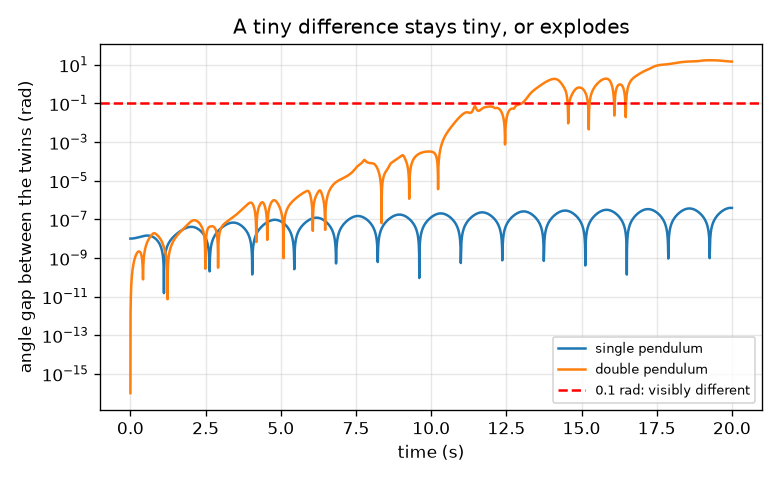
\includegraphics[width=0.85\linewidth]{figures/s01_gap_growth.png}\\\small Angle gap on a log axis: flat for the single pendulum, an explosion for the double pendulum.\end{center}

\subsection*{E. Worked example}
A 1 m pendulum swings through a small angle. Find its swing time from the formula and compare it with the simulation.
\begin{enumerate}[nosep]
\item The formula is T = 2 pi sqrt(L / g) with L = 1 m and g = 9.81 m/s\textasciicircum{}2.
\item L / g = 1 / 9.81 = 0.10194 s\textasciicircum{}2, and its square root is 0.31928 s.
\item T = 2 pi x 0.31928 = 2.0061 s.
\item The simulation with a 2 degree release, measured from the time the pendulum returns to its release point, gives 2.006 s.
\item Sanity check: a pendulum about one metre long ticks roughly once every two seconds, as in a grandfather clock (a 'seconds pendulum' beats seconds, so one full swing there takes 2 s).
\end{enumerate}
\textbf{Answer.} T = 2.006 s from the formula and 2.006 s from the simulation.

\subsection*{F. Questions}
\begin{enumerate}[nosep]
\item \textbf{Conceptual.} A friend says: the double pendulum moves randomly, so no equation can describe it. Explain what is right and what is wrong in that sentence.
\item \textbf{Numerical.} Find the swing time of a pendulum 0.25 m long with the formula T = 2 pi sqrt(L / g). Is it more or less than the 1 m pendulum, and by what factor?
\item \textbf{Graph and simulation interpretation.} On the gap graph, the double pendulum's gap grows from 3.2e-4 rad at 10 s to 0.62 rad at 15 s. By what factor does it grow in those 5 s, and what is the growth rate per second?
\item \textbf{Design and optimisation challenge.} Design: you may measure the starting angle with a protractor of precision 1e-3 rad. Using a growth rate of 1.5 per second, how long can you forecast to within 0.1 rad? What precision would 10 s need? State your assumption.
\end{enumerate}

\section{Session 2: Equations, energy and a trustworthy simulation}

\subsection*{A. Real-world problem}
Before anyone believes your simulation you must be able to check it. For a double pendulum there is no formula for the motion, but two things are certain: with no friction the total energy (movement plus height) must stay constant, and for tiny swings the motion must reduce to two simple patterns whose frequencies can be calculated by hand. A weather office or a robot-arm maker runs exactly such tests before trusting a model. Which time step is small enough, and how do we know?

\subsection*{B. Concept and theory}
Take two point masses m1 and m2 on rods of lengths l1 and l2, with angles theta1 and theta2 from straight down. The Lagrangian method (kinetic energy minus potential energy, with the angles as coordinates) gives two coupled equations for the angular accelerations; they are written out below and also in matrix form, M(theta) theta'' = force terms, which we use as an independent check. The total energy E = T + V is constant. For small angles sin x is about x and cos x about 1, so the equations become linear, M theta'' = -K theta, and the motion is a sum of two normal modes: patterns in which both rods swing at one common frequency w. The frequencies satisfy det(K - w\textasciicircum{}2 M) = 0. For equal masses and rods w\textasciicircum{}2 = (g / l)(2 -/+ sqrt 2), that is 2.397 rad/s (rods swing in the same direction, the lower one 1.414 times as far) and 5.787 rad/s (rods swing in opposite directions). To advance the motion in time we use RK4 with step h; its error per unit time is proportional to h\textasciicircum{}4, so halving h should cut an error by about 16.

\begin{itemize}[nosep]
\item theta1, theta2: angles of the upper and lower rod from straight down (rad)
\item omega1, omega2: angular speeds (rad/s)
\item m1, m2: masses of the two balls (kg)
\item l1, l2: lengths of the two rods (m)
\item g: gravity (9.81) (m/s\textasciicircum{}2)
\item T, V, E: kinetic, potential and total energy (height measured from the pivot) (J)
\item E\_ref: energy scale (m1 + m2) g l1 + m2 g l2 (J)
\item h: time step of the solver (s)
\item w: normal-mode frequency of small swings (rad/s)
\end{itemize}

\begin{equation*}
\ddot\theta_1=\frac{-g(2m_1+m_2)\sin\theta_1-m_2g\sin(\theta_1-2\theta_2)-2\sin(\theta_1-\theta_2)\,m_2\left(\dot\theta_2^{2}l_2+\dot\theta_1^{2}l_1\cos(\theta_1-\theta_2)\right)}{l_1\left(2m_1+m_2-m_2\cos(2\theta_1-2\theta_2)\right)}
\end{equation*}

\begin{equation*}
\ddot\theta_2=\frac{2\sin(\theta_1-\theta_2)\left(\dot\theta_1^{2}l_1(m_1+m_2)+g(m_1+m_2)\cos\theta_1+\dot\theta_2^{2}l_2m_2\cos(\theta_1-\theta_2)\right)}{l_2\left(2m_1+m_2-m_2\cos(2\theta_1-2\theta_2)\right)}
\end{equation*}

\begin{equation*}
T=\tfrac12(m_1+m_2)l_1^2\dot\theta_1^2+\tfrac12m_2l_2^2\dot\theta_2^2+m_2l_1l_2\dot\theta_1\dot\theta_2\cos(\theta_1-\theta_2),\qquad V=-(m_1+m_2)gl_1\cos\theta_1-m_2gl_2\cos\theta_2
\end{equation*}

\begin{equation*}
\det(K-\omega^{2}M)=0,\quad M=\begin{pmatrix}(m_1+m_2)l_1^2 & m_2l_1l_2\\ m_2l_1l_2 & m_2l_2^2\end{pmatrix},\ K=\begin{pmatrix}(m_1+m_2)gl_1 & 0\\ 0 & m_2gl_2\end{pmatrix}
\end{equation*}

\begin{equation*}
\omega^{2}=\frac{g}{l}\left(2\mp\sqrt{2}\right)\quad\text{(equal masses and rods)}
\end{equation*}

\begin{center}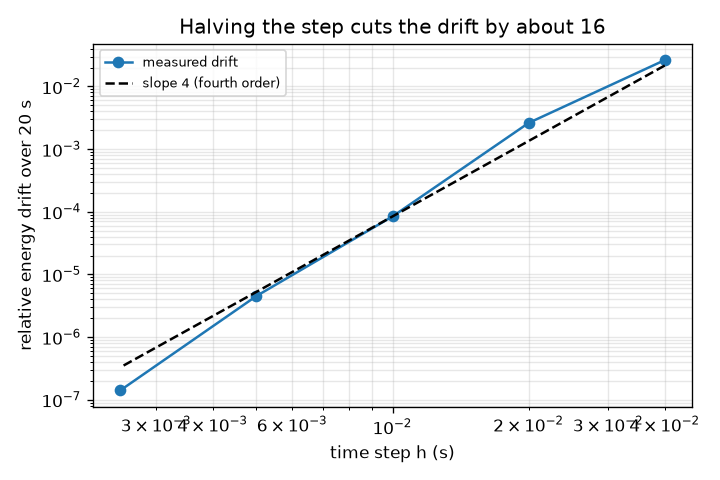
\includegraphics[width=0.85\linewidth]{figures/s02_drift_vs_step.png}\\\small Energy drift over 20 s against step size: close to the slope-4 line of a fourth-order method.\end{center}

\subsection*{E. Worked example}
For equal masses (1 kg) and equal rods (1 m), find the two small-swing frequencies and periods, and check them against a simulation of amplitude 0.001 rad.
\begin{enumerate}[nosep]
\item For equal masses and rods w\textasciicircum{}2 = (g / l)(2 -/+ sqrt 2) with g / l = 9.81 s\textasciicircum{}-2 and sqrt 2 = 1.4142.
\item Slow mode: w\textasciicircum{}2 = 9.81 x 0.5858 = 5.747 s\textasciicircum{}-2, so w = 2.397 rad/s and the period is 2 pi / 2.397 = 2.621 s.
\item Fast mode: w\textasciicircum{}2 = 9.81 x 3.4142 = 33.49 s\textasciicircum{}-2, so w = 5.787 rad/s and the period is 2 pi / 5.787 = 1.086 s.
\item Mode shapes: theta2 / theta1 = +1.414 for the slow mode and -1.414 for the fast mode.
\item Start the simulation at rest with theta1 = 0.001 rad and theta2 = 0.001414 rad (slow mode): over 3 s the largest difference from 0.001 cos(2.397 t) is 8.9e-10 rad; for the fast mode it is 4.5e-8 rad. The nonlinear model agrees with the hand result to far better than 1e-6 rad.
\end{enumerate}
\textbf{Answer.} Frequencies 2.397 and 5.787 rad/s (periods 2.621 s and 1.086 s); the simulation matches to better than 1e-7 rad.

\subsection*{F. Questions}
\begin{enumerate}[nosep]
\item \textbf{Conceptual.} If a simulation keeps the total energy constant to 1e-9, does that prove it is correct? What else would you test?
\item \textbf{Numerical.} Find the total energy of a double pendulum with m1 = m2 = 1 kg, l1 = l2 = 1 m, released from rest with both rods at 60 degrees. Then repeat for 90 degrees. Give units and say whether the signs make sense.
\item \textbf{Graph and simulation interpretation.} On the drift-versus-step graph, which of the tested steps keeps the energy error below 1e-5 over 20 s, and by about what factor does the error fall when you halve h from 0.01 s to 0.005 s?
\item \textbf{Design and optimisation challenge.} Design: choose a step for a 20 s run released at 120 degrees with energy error below 1e-6. Compare the cost with the step that gives 1e-5. State the trade-off.
\end{enumerate}

\section{Session 3: Measuring chaos and the limits of forecasting}

\subsection*{A. Real-world problem}
Weather models, satellite orbits and robot arms all meet the same wall: a tiny error in the starting measurement grows until the forecast is useless. The double pendulum shows it on a table top. Today we ask the quantitative questions. How fast does a tiny error grow? For which starts is the motion regular and for which chaotic? And if a lab can measure the start to 1e-6 rad, for how many seconds can the forecast be trusted?

\subsection*{B. Concept and theory}
Two solvers are compared. RK4 is very accurate over a short time but leaks energy steadily. The implicit midpoint rule, applied to the Hamiltonian form with positions and momenta, is symplectic: its energy error does not grow however long we run, though it is larger at first (it is only second order). For sensitivity, start two copies delta0 apart and track the distance d(t) between them in the four-dimensional space of angles and angular speeds. While d is small, d(t) is about delta0 exp(lambda t), so ln d is a straight line against t whose slope is the largest Lyapunov exponent lambda (units 1/s). A positive lambda means chaos. The line stops when d is as large as the motion itself (saturation), so we fit only between d = 1e-6 and 1e-2. The Benettin method pulls the twin back to distance delta0 every 0.1 s and averages the logarithm of the growth. Both estimates belong to one start only: lambda depends on the initial condition, and near zero it cannot be told from zero in a finite run. The flip-time map releases the pendulum from rest on a grid of (theta1, theta2) and records when the outer rod first goes over the top; stripes and speckles mark chaos. Validation by energy: kinetic energy is never negative, so the outer rod can reach the top only if the energy E = -2 g cos(theta1) - g cos(theta2) is at least -g, so any start with 2 cos(theta1) + cos(theta2) \textgreater{} 1 can never flip. Finally, if the start error is delta0 and we accept an error Delta, the forecast fails at t = ln(Delta / delta0) / lambda.

\begin{itemize}[nosep]
\item delta0: size of the start error (rad (or mixed rad and rad/s))
\item d(t): distance between the two runs in angle and angular-speed space (mixed rad and rad/s)
\item lambda: largest Lyapunov exponent (1/s)
\item Delta: largest forecast error we accept (0.1) (rad)
\item t\_h: predictability horizon (s)
\item h: time step (s)
\item E: total energy, equal to -2 g cos(theta1) - g cos(theta2) for a rest start (J)
\item q, p: positions (angles) and momenta of the Hamiltonian form (rad, kg m\textasciicircum{}2/s)
\end{itemize}

\begin{equation*}
d(t)\approx\delta_0\,e^{\lambda t}\ \Longleftrightarrow\ \ln d(t)=\ln\delta_0+\lambda t
\end{equation*}

\begin{equation*}
\lambda\approx\frac1T\sum_{k}\ln\frac{d_k}{\delta_0}\quad\text{(Benettin: the gap is reset to }\delta_0\text{ after each interval)}
\end{equation*}

\begin{equation*}
z_{n+1}=z_n+h\,F\!\left(\tfrac12(z_n+z_{n+1})\right),\qquad \dot q=M^{-1}p,\ \ \dot p=-\partial_qH
\end{equation*}

\begin{equation*}
2\cos\theta_1+\cos\theta_2>1\ \Longrightarrow\ E<-g\ \Longrightarrow\ \text{the outer rod cannot flip}
\end{equation*}

\begin{equation*}
t_h=\frac{1}{\lambda}\ln\frac{\Delta}{\delta_0}
\end{equation*}

\begin{center}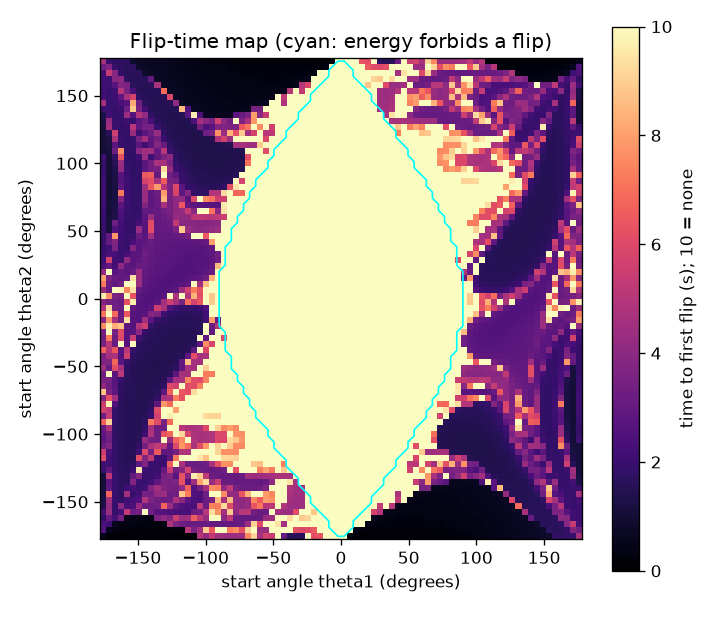
\includegraphics[width=0.85\linewidth]{figures/s03_flip_time_map.png}\\\small Flip-time map of 80 x 80 rest starts; the cyan outline marks where energy forbids a flip.\end{center}

\subsection*{E. Worked example}
A lab measures the starting angles of a double pendulum to 1e-6 rad. If lambda = 1.4 per second and we accept an error of 0.1 rad, how long is the forecast good? How much longer if the measurement is a thousand times better?
\begin{enumerate}[nosep]
\item t\_h = ln(Delta / delta0) / lambda = ln(0.1 / 1e-6) / 1.4 = ln(100000) / 1.4.
\item ln(100000) = 11.513, so t\_h = 11.513 / 1.4 = 8.22 s.
\item With delta0 = 1e-9: ln(1e8) = 18.421, so t\_h = 18.421 / 1.4 = 13.16 s.
\item The gain is ln(1000) / 1.4 = 6.908 / 1.4 = 4.93 s: a thousand times better instruments buy about five seconds.
\item Check with the simulation for the 120 degree release: the Benettin lambda is 1.43 per second, so the formula gives 8.05 s, and a forecast started 1e-6 rad off in theta1 fails (0.1 rad) at 10.2 s. The median over random error directions is 10.3 s, a factor 1.3 longer than the formula; with 1e-9 the median is 16.8 s (gain 6.5 s).
\end{enumerate}
\textbf{Answer.} About 8.2 s with 1e-6 rad (formula; 10 s measured for this start) and only about 5 to 7 s more with a thousand times better measurement.

\subsection*{F. Questions}
\begin{enumerate}[nosep]
\item \textbf{Conceptual.} A colleague proposes to forecast a chaotic system for twice as long by buying a measuring device twice as precise. Explain why this does not work and what would be needed instead.
\item \textbf{Numerical.} For lambda = 1.2 per second, a start error of 1e-8 rad and an accepted error of 0.5 rad, find the predictability horizon. Give the units and a sanity check.
\item \textbf{Graph and simulation interpretation.} In Figure 2 the straight segment rises from d = 1e-6 at 3.7 s to d = 1e-2 at 10.3 s, while the least-squares fit over that window gives lambda = 1.21 per second and the Benettin method 1.43 per second. Estimate lambda from the two end points, and explain why the three numbers differ.
\item \textbf{Design and optimisation challenge.} Design: you want a 15 s forecast within 0.1 rad for the 120 degree release (lambda about 1.43 per second). What start precision does the formula demand? Is it realistic for a rotary encoder of 1e-5 rad resolution? What would you do instead?
\end{enumerate}

\section{Real-world mini-project}
\textbf{How long can you forecast a double pendulum?.} A lab can measure the two starting angles of a double pendulum to within 1e-6 rad. Released from rest with both rods at 100, 120 or 140 degrees, for how long does a forecast stay within 0.1 rad of the true motion? Use \texttt{benettin}, \texttt{predicted\_horizon} and \texttt{median\_horizon} from Session 3 (20 random error directions, seed 7).

\section{The path ahead}
\begin{enumerate}[nosep]
\item \textbf{Session 4: A fourth-order symplectic solver.} A solver whose energy error stays bounded and small at a coarse step.
\item \textbf{Session 5: The full Lyapunov spectrum.} All four exponents of the 120 degree release instead of the largest one only.
\item \textbf{Session 6: Ensemble forecasts.} 1000 forecasts from a Gaussian cloud of start errors of 1e-6 rad.
\item \textbf{Session 7: A damped, real pendulum.} A damped model and a fit routine run on a synthetic measurement.
\item \textbf{Session 8: Chaos for unequal masses.} Flip-time maps for general masses and rods.
\end{enumerate}

\section{Answers and hints}

\subsection*{Session 1}
\begin{enumerate}[nosep]
\item \textbf{Conceptual.} Hint: Ask whether the same start always gives the same motion, and what the gap graph shows about the start. Solution: The motion looks random but is not: the equations are exact and the same start always gives the same motion (it is deterministic). What is true is that the motion is extremely sensitive to the start: a difference of 1e-8 rad grows to more than 0.1 rad in about 13 s, so we cannot predict it far ahead unless we know the start almost perfectly. Chaos means unpredictable in practice, not lawless.
\item \textbf{Numerical.} Hint: Put L = 0.25 m and g = 9.81 m/s\textasciicircum{}2 into the formula; then compare with 2.006 s. Solution: L / g = 0.25 / 9.81 = 0.02548 s\textasciicircum{}2, sqrt = 0.1596 s, T = 2 pi x 0.1596 = 1.003 s. It is half of 2.006 s: four times shorter gives half the swing time (T goes as the square root of L). Units: seconds.
\item \textbf{Graph and simulation interpretation.} Hint: Divide the two gaps, then take the natural logarithm and divide by 5 s. Solution: The factor is 0.62 / 3.2e-4 = about 1950. The natural logarithm of 1950 is 7.58, so the rate is 7.58 / 5 s = 1.5 per second (the gap multiplies by about 4.5 every second). This rate, called the Lyapunov exponent, is measured properly in Session 3.
\item \textbf{Design and optimisation challenge.} Hint: The gap is about delta x exp(1.5 t); solve for t when it reaches 0.1, then solve for delta at t = 10 s. Solution: From delta e\textasciicircum{}(1.5 t) = 0.1 we get t = ln(0.1 / 1e-3) / 1.5 = ln(100) / 1.5 = 4.605 / 1.5 = 3.1 s. For 10 s we need delta = 0.1 e\textasciicircum{}(-15) = 3e-8 rad, thirty thousand times better than the protractor. Assumption: the growth is a clean exponential from the start; the real gap grows more slowly at first (see the graph), so these numbers are rough. Trade-off: each extra second of forecast needs the start known e\textasciicircum{}1.5 = 4.5 times better.
\end{enumerate}

\subsection*{Session 2}
\begin{enumerate}[nosep]
\item \textbf{Conceptual.} Hint: Think of a simulation that moves the pendulum on the right energy shell but at the wrong speed. Solution: No. Energy conservation is necessary, not sufficient: a solver could keep E constant and still get the timing (phase) of the swing wrong, or solve slightly different equations that also conserve a similar energy. We also compare with cases that have a known answer: the small-angle normal modes, hanging at rest, and an independent form of the equations (mass-matrix form), and we check that the error shrinks as the step shrinks.
\item \textbf{Numerical.} Hint: At rest T = 0 and V = -(m1 + m2) g l1 cos(theta1) - m2 g l2 cos(theta2) with equal angles. Solution: V = -3 g cos(theta) with g = 9.81. At 60 degrees cos = 0.5 so E = -14.715 J; at 90 degrees cos = 0 so E = 0 J. Height is measured from the pivot, so hanging below the pivot is negative energy; at 90 degrees the balls are level with the pivot, zero height. Hanging at rest is the lowest energy, -3 g = -29.43 J.
\item \textbf{Graph and simulation interpretation.} Hint: Read the points at 0.01 s and 0.005 s, then divide. Solution: The error is 8.4e-5 at 0.01 s (too large) and 4.5e-6 at 0.005 s (below 1e-5). Halving the step cuts it by 8.4e-5 / 4.5e-6 = 18.6, close to the 2\textasciicircum{}4 = 16 expected for a fourth-order method.
\item \textbf{Design and optimisation challenge.} Hint: Use largest\_step(1e-6, ...) with the candidates 0.04, 0.02, 0.01, 0.005, 0.0025 s. Solution: 0.0025 s gives 1.4e-7 (passes) and 0.005 s gives 4.5e-6 (fails 1e-6, passes 1e-5). So 0.0025 s for 1e-6 needs 8000 steps, against 4000 steps with 0.005 s for 1e-5: twice the work for 30 times less error. RK4 makes four rate evaluations per step, so 32000 against 16000. Trade-off: accuracy against run time; also, for a chaotic motion extra accuracy extends how long the run follows the true path only slowly (Session 3).
\end{enumerate}

\subsection*{Session 3}
\begin{enumerate}[nosep]
\item \textbf{Conceptual.} Hint: Use t\_h = ln(Delta / delta0) / lambda. Solution: The horizon depends on the logarithm of the precision: halving delta0 adds only ln 2 / lambda, about 0.5 s for lambda = 1.4 per second. To double a 10 s horizon you would need delta0 about e\textasciicircum{}14 = a million times smaller. Better options are to accept a larger error Delta (which also helps only logarithmically), to forecast statistics (averages and probabilities) instead of the exact path, or to correct the forecast with new measurements as time goes on.
\item \textbf{Numerical.} Hint: t\_h = ln(Delta / delta0) / lambda. Solution: Delta / delta0 = 0.5 / 1e-8 = 5e7, ln(5e7) = 17.73, so t\_h = 17.73 / 1.2 = 14.8 s. Sanity check: with delta0 = 1e-8 and Delta = 0.1 the earlier simulation passed 0.1 rad at about 13 s; a larger tolerance and slightly smaller lambda give a bit more, so 15 s is plausible.
\item \textbf{Graph and simulation interpretation.} Hint: Slope of ln d: ln(1e-2 / 1e-6) divided by the time between the two points. Solution: ln(1e4) = 9.21 over 6.6 s gives 1.40 per second. The fit (1.21) and Benettin (1.43) differ because the growth rate is not constant along the orbit: the pendulum alternates between phases of fast and slow stretching, so a finite-time estimate depends on the window and the length of the run. Quote lambda with this uncertainty (here about 1.2 to 1.5 per second) and say for which start it was measured.
\item \textbf{Design and optimisation challenge.} Hint: Solve t\_h = 15 s for delta0: delta0 = Delta exp(-lambda t\_h). Solution: delta0 = 0.1 exp(-1.43 x 15) = 0.1 exp(-21.45) = 4.8e-11 rad, a million times finer than a 1e-5 rad encoder, which would give only about 5 s by the formula. It is not realistic. Alternatives: shorten the horizon you promise, accept 1 rad error (gain ln(10) / 1.43 = 1.6 s only), use repeated measurements to correct the forecast, or forecast the probability of a flip rather than the path. Assumption: friction and the model error are neglected, which would make things worse in reality.
\end{enumerate}

\section{How to join}
Read \texttt{CONTRIBUTING.md} in the repository, then pick an issue labelled \texttt{good first issue}. Repository: \url{https://github.com/KrunalPanchal1995/openchaos}

\end{document}
